\documentclass[12pt]{article}
\usepackage[a4paper]{geometry}
\usepackage{fullpage}
\usepackage[T1]{fontenc}
\usepackage[utf8]{inputenc}
\usepackage{graphicx}
\usepackage{mathpazo}
\pagenumbering{gobble}
\usepackage{siunitx}
\DeclareSIUnit\voltampere{VA}
\usepackage{amsmath}
\usepackage[spanish]{babel}
\usepackage{steinmetz}
\usepackage{enumitem}
\renewcommand{\thesection}{Problema \arabic{section}}

\begin{document}

\title{}

\date{2019-20}

\section{}
En el circuito de la figura los valores se dan en voltios y ohmios, según corresponda. Determinar el valor de la intensidad I aplicando la propiedad de proporcionalidad.

\begin{center}
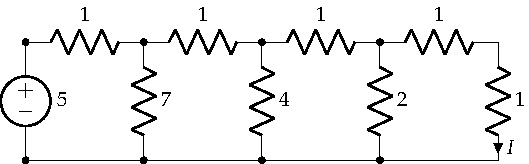
\includegraphics{figs/proporcionalidad}
\end{center}

\noindent\hrulefill

Suponiendo que $I = \SI{1}{\ampere}$, resolvemos el circuito hacia el generador. Obtenemos $\epsilon = \SI{11}{\volt}$. Por tanto, con un generador de $\SI{5}{\volt}$ la corriente será $I = \SI[parse-numbers=false]{5/11}{\ampere}$ (regla de tres simple).


\section{}

En el circuito de la figura determina:
\begin{itemize}
\item $u_R(t)$  y $u_L(t)$.
\item Balance de potencias.
\end{itemize}

\begin{center}
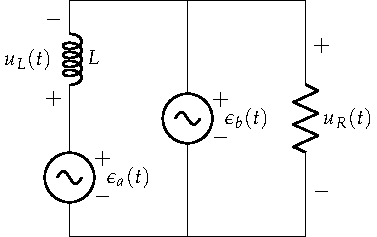
\includegraphics{figs/superposicion2}
\end{center}


Datos:
\begin{align*}
  e_a(t) &= \SI[parse-numbers=false]{3\sqrt{2} \sin(10^3 t)}{\volt}\\
  e_b(t) &= \SI[parse-numbers=false]{30\sqrt{2} \sin(10^4 t)}{\volt}\\
  R &= \SI{30}{\ohm}\\
  L &= \SI{3}{\milli\henry}
\end{align*}


\noindent\hrulefill

% \begin{center}
% 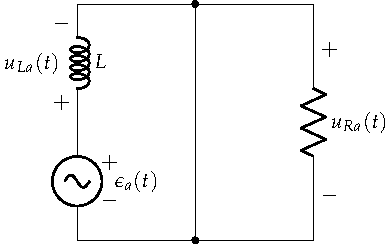
\includegraphics{figs/superposicion2_A}
% \end{center}

% \begin{center}
% 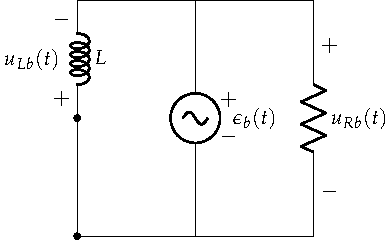
\includegraphics{figs/superposicion2_B}
% \end{center}

\clearpage

\section{}

El circuito de la figura se encuentra en régimen permanente. Determina
analíticamente la expresión de $i(t)$, así como las potencias entregadas por los
generadores y disipadas por las resistencias $R_1$, y $R_2$.
\begin{center}
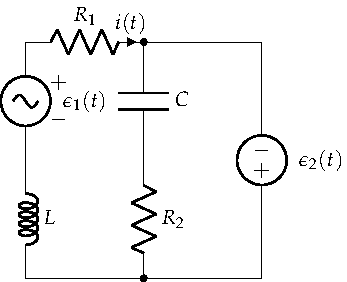
\includegraphics{figs/superposicion1}
\end{center}

Datos:
\begin{align*}
  e_1(t) &= \SI[parse-numbers=false]{50 \sin(1000 t)}{\volt}\\
  e_2(t) &= \SI{30}{\volt}\\
  R_1 &= \SI{6}{\ohm}\\
  R_2 &= \SI{6}{\ohm}\\
  L &= \SI{8}{\milli\henry}\\
  C &= \SI{10}{\micro\farad}
\end{align*}


\noindent\hrulefill

\clearpage

\section{}

En el circuito de la figura el generador de tensión $e(t)$ es de onda cuadrada simétrica, tal y como se muestra en la figura. La potencia total disipada por las resistencias $R_1$ y $R_2$ es de $\SI{40}{\watt}$.
Determina:

\begin{itemize}
  \item Valor máximo $E_0$ de la onda cuadrada.
  \item Forma de onda de la tensión $u(t)$ y su valor eficaz.
  \item Potencias disipadas en $R_1$ y $R_2$ si la frecuencia de la onda $e(t)$ aumenta al doble.
\end{itemize}

\begin{center}
  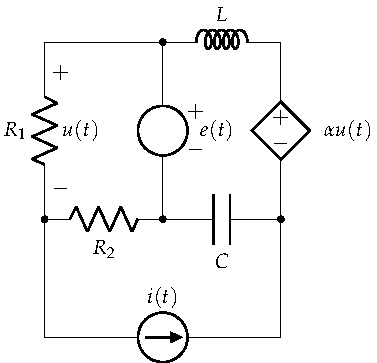
\includegraphics{figs/superposicion3}
  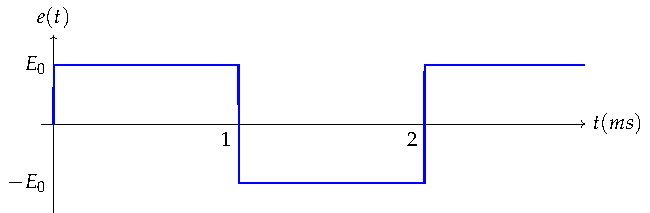
\includegraphics{figs/superposicionOndaCuadrada}
\end{center}
Datos:

\begin{align*}
  i(t) &= \SI{1}{\ampere}\\
  R_1 &= \SI{60}{\ohm}\\
  R_2 &= \SI{40}{\ohm}\\
  L &= \SI{10}{\milli\henry}\\
  C &= \SI{1}{\micro\farad}
\end{align*}

\noindent\hrulefill

\clearpage

\section{}

Obtén los generadores equivalentes de Thévenin y Norton del circuito de la figura respecto de A y B.

\begin{center}
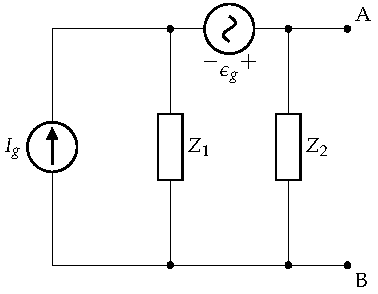
\includegraphics{figs/Thevenin3}
\end{center}

Datos:
\begin{align*}
  \overline{\epsilon_g} &= \SI[parse-numbers=false]{32 + 12j}{\volt}\\
  \overline{I} &= \SI[parse-numbers=false]{2\phase{0}}{\ampere}\\
  \overline{Z}_1 &= \SI[parse-numbers=false]{8 - 6j}{\ohm}\\
  \overline{Z}_2 &= \SI[parse-numbers=false]{8 + 6j}{\ohm}
\end{align*}

\noindent\hrulefill

\clearpage

\section{}

Obtén el generador equivalente de Thévenin del circuito de la figura respecto de A y B.
\begin{center}
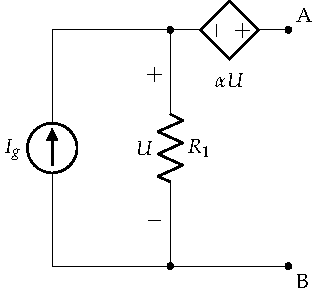
\includegraphics{figs/Thevenin1}
\end{center}

\noindent\hrulefill

\clearpage

\section{}

Obtén el generador equivalente de Thévenin del circuito de la figura respecto de A y B.

\begin{center}
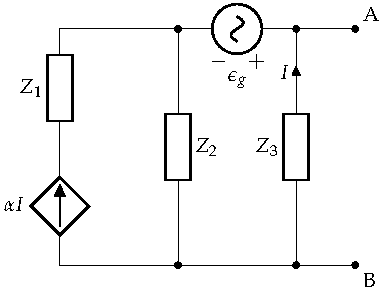
\includegraphics{figs/Thevenin4}
\end{center}

Datos:
\begin{align*}
  \overline{\epsilon_g} &= \SI[parse-numbers=false]{12 - 16j}{\volt}\\
  \overline{Z}_1 &= \SI[parse-numbers=false]{1 - j}{\ohm}\\
  \overline{Z}_2 &= \SI[parse-numbers=false]{1 + j}{\ohm}\\
  \overline{Z}_3 &= \SI[parse-numbers=false]{5 + 3j}{\ohm}\\
  \alpha &= 2
\end{align*}

\noindent\hrulefill

\clearpage

\section{}

Obtén el generador equivalente de Thévenin del circuito de la figura respecto de A y B. A partir de este generador, calcula la resistencia a colocar en AB para obtener la máxima potencia, calculando esta potencia y la potencia entregada por el generador $\epsilon$.

\begin{center}
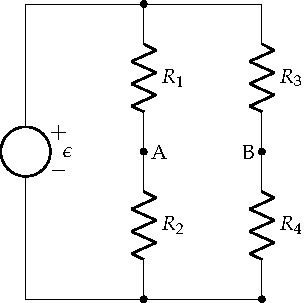
\includegraphics{figs/Thevenin2}
\end{center}

Datos:

\begin{align*}
  \epsilon &= \SI{54}{\volt}\\
  R_1 = R_4 &= \SI{8}{\ohm}\\
  R_2 = R_3 &= \SI{10}{\ohm}
\end{align*}

\noindent\hrulefill

\clearpage

\section{}

Obtén el generador equivalente de Thévenin del circuito de la figura respecto de A y B. A partir de este generador, calcula la impedancia a colocar en AB para obtener la máxima potencia, calculando esta potencia.

\begin{center}
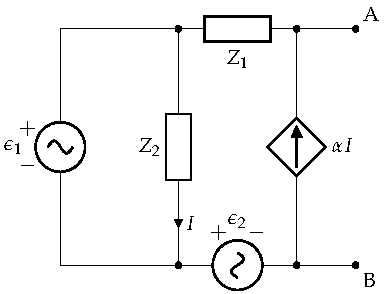
\includegraphics{figs/Thevenin5}
\end{center}

Datos:
\begin{align*}
  \overline{\epsilon_1} &= \SI[parse-numbers=false]{10\phase{0}}{\volt}\\
  \overline{\epsilon_2} &= \SI[parse-numbers=false]{10j}{\volt}\\
  \overline{Z}_1 &= \SI[parse-numbers=false]{4 - 3j}{\ohm}\\
  \overline{Z}_2 &= \SI[parse-numbers=false]{3 + 4j}{\ohm}\\
  \alpha &= 2
\end{align*}

\noindent\hrulefill

\end{document}